\section{Quantized energy level of atom}
So far we have trated the atom semi-clasically. We will now describe the atomic degree of freedom-
electrons as quantum mechanics objects.
The Hamiltonian and eigenequation for a single $e^-$ in the atom are:
\begin{align}
    \hH_A=\frac{\hp^2}{2m}+V(\hbr),\quad\hH_A\ket{\psi_n}=E_n\ket{\psi_n}.
\end{align}
Not that $\ket{\psi_n}$ is not a position eigenstate, since $\hH_0$ contains both $\hbr$ and $\hbp$ operators.

The electronic wavefunction fo an $e^-$ in the state $\ket{\psi_n}$ is given by $\braket{\br|\psi_n}=\psi_n(\br)$.

Let us consider two-energy eigenstates:
\begin{align}
    \underbrace{\ket{\psi_g}=\ket{g}}_{\text{ground}}\quad\text{and}\quad\underbrace{\ket{\psi_e}=\ket{e}}_{\text{excited}}.
\end{align}
We restrict out attention to two-energy levels since they might have a stronger posibility of transition between them.

We would like to express the dipole operator in the energy basis:
\begin{align*}
    \braket{g|\hbd|e}&=-e\braket{g|\hbr|e}=-e\int d^3r\;\int d^3r'\;\braket{g|\br}\braket{\br|\hbr'|\br'}\braket{\br'|e}=-e\int d^3r\;\br\psi_g^*(\br)\psi_e(\br)=\bd_{ge}.
\end{align*}
Thus, the dipole transition matrix corresponds to the overlap between the electronic wavefunction in two energy levels. Similarly,
\begin{align*}
    \braket{e|\hbd|g}*=-e\int d^3r\;\br\psi_g(\br)\psi_e^*(\br)=\bd_{eg}=\bd_{ge}^*,\quad
    \braket{g|\hbd|g}=\braket{e|\hbd|e}=0
\end{align*}
The dipole matrix is symmetric. We can thus express the dipole operator as:
\begin{align}
    \hbd=\bd_{eg}\ket{e}\bra{g}+\bd_{ge}\ket{g}\bra{e}=\bd\hsigma_++\bd^*\hsigma_-,
\end{align}
where $\hsigma$ operators are Pauli matrices and corresponds to atomic raising and lowering atomic operators, respectively.

The free Hamiltonian of the atom $\hH_0$ can be expressed in terms of its energy eigenstates:
\begin{align*}
    \hH_0=\sum-nE_n\ket{n}\bra{n}=E_g\ket{g}\bra{g}+E_e\ket{e}\bra{e}=\hbar\omega_0\ket{e}\bra{e}\quad(E_g=0\land E_e=\hbar\omega_0)=\hbar\omega_0\hsigma_+\hsigma_-
\end{align*}
The total Hamiltonian of an atom interacting with quantized EM-field is:
\begin{align}
    \hH_{tot}=\underbrace{\hH_A}_{\text{atom}}+\underbrace{\hH_F}_{\text{field}}+\underbrace{\hH_{int}}_{\text{interaction}},
\end{align}
where 
\begin{align}
    \hH_A&=\hbar\omega_0\ket{e}\bra{e}=\hbar\omega_0\hsigma_+\hsigma_0,\\
    \hH_F&=\sum_{\bk,\lambda}\hbar\omega_{\bk}\left(\ha_{\bk,\lambda}\ha_{\bk,\lambda}+\frac{1}{2}\right),\quad[\ha_{\bk,\lambda},\ha^\dagger_{\bk,\lambda}]=1,\\
    \hH_{int}&=-\hbd\cdot\hbE(\br_A),\quad
    \begin{array}{l}
        \hbd=\bd\ket{e}\bra{g}+\bd^*\ket{g}\bra{e}=\bd\hsigma_++\bd^*\hsigma_-,\\    
        \hbE(\br_A)=i\sum_{\bk,\lambda}\he_{\bk,\lambda}\sqrt{\frac{\hbar\omega_{\bk}}{2\varepsilon_0V}}[\ha_{\bk,\lambda}e^{i\bk\cdot\br_A}-\ha^\dagger_{\bk,\lambda}
    e^{-i\bk\cdot\br_A}].
    \end{array}
\end{align}
We now move to the interaction picture where we define $H_{tot}=H_0+H_{int}$. In Schrodinger picture,
\begin{align*}
    i\hbar\partial_t\ket{\psi}_s=(H_0+H_{int})\ket{\psi}_s
\end{align*}
In the interaction picture we define 
\begin{align*}
    \ket{\psi}_I=e^{iH_0t/\hbar}\ket{\psi}_s,
\end{align*}
and 
\begin{align*}
    i\hbar\partial_t\ket{\psi}_I&=i\hbar\partial_t[e^{iH_0t/\hbar}\ket{\psi}_s]=i\hbar\frac{iH_0}{\hbar}e^{iH_0t/\hbar}\ket{\psi}_s+i\hbar e^{iH_0t/\hbar}\partial_t\ket{\psi}_s\\
    &=-H_0\cancel{e^{iH_0t/\hbar}}\ket{\psi}_s+e^{iH_0t/\hbar}(\cancel{H_0}+H_{int})\ket{\psi}_s=\underbrace{e^{iH_0t/\hbar}H_{int}e^{-iH_0t/\hbar}}_{H_{int,T}\text{ or }\tilde{H}_{int}}
    \underbrace{e^{iH_0t/\hbar}\ket{\psi}_s}_{\ket{\psi}_I}\\
    i\hbar\partial_t\ket{\psi}_I&=\tilde{H}_{int}\ket{\psi}_I.
\end{align*}
Let us consider the interaction Hamiltonian in interaction picture:
\begin{align*}
    \tilde{H}_{int}&=e^{iH_0t/\hbar}\hH_{int}e^{-iH_0t/\hbar}=e^{iH_0t/\hbar}[-\hbd\cdot\hbE(\br_A)]e^{-iH_0t/\hbar}\\
    \tilde{H}_{int}&=-e^{i(H_A+H_F)t/\hbar}(\bd\hsigma_++\bd^*\hsigma_-)\cdot i\sum_{\bk,\lambda}\he_{\bk,\lambda}\sqrt{\frac{\hbar\omega_{\bk}}{2\varepsilon_0V}}
    [\ha_{\bk,\lambda}e^{i\bk\cdot\br}-\ha^\dagger_{\bk,\lambda}e^{-i\bk\cdot\br}]e^{-i(H_A+H_F)t/\hbar}.
\end{align*}
In solving the above, we encounter 
\begin{align*}
    &e^{iH_At/\hbar}\hsigma_+e^{-iH_At/\hbar}=\hsigma_+e^{i\omega_0t},\quad
    e^{iH_At/\hbar}\hsigma_-e^{-iH_At/\hbar}=\hsigma_-e^{-i\omega_0t},\\
    &e^{iH_Ft/\hbar}\ha_{\bk,\lambda}e^{-iH_Ft/\hbar}=\ha_{\bk,\lambda}e^{-i\omega_{\bk}t},\quad
    e^{iH_Ft/\hbar}\ha^\dagger_{\bk,\lambda}e^{-iH_Ft/\hbar}=\ha^\dagger_{\bk,\lambda}e^{i\omega_{\bk}t}.
\end{align*}
We then have:
\begin{align*}
    \tilde{H}_{int}=-(\bd\hsigma_+e^{i\omega_0t}+\bd^*\hsigma_-e^{-i\omega_0t})\cdot i\sum_{\bk,\lambda}\he_{\bk,\lambda}
    \sqrt{\frac{\hbar\omega_{\bk}}{2\varepsilon_0V}}\left[\ha_{\bk,\lambda}e^{i(\bk\cdot\br-\omega_{\bk}t)}-\ha^\dagger_{\bk,\lambda}e^{-i(\bk\cdot\br-\omega_{\bk}t)}\right].
\end{align*}

\bfemph{Rotating wave approximation (RWA)}: Terms $e^{\pm i(\omega_0+\omega_n)t}$ oscillate on timescales of $\sim10^{-15}\;s$.
On typical observation timescales $\sim1\;ns$ and it contains about $(\omega_0+\omega_{\bk})t\sim10^{-15}\cdot10^{-9}\sim10^8$ oscillations. 
Thus, these fast-oscilating terms averages to zero.

Under the RWA, the interaction Hamiltonian becomes:
\begin{align*}
    \tilde{H}_{int}\approx\sum_{\bk,\lambda}-i\bd\cdot\he_{\bk,\lambda}\sqrt{\frac{\hbar\omega_{\bk}}{2\varepsilon_0V}}\left[
        \hsigma_+\ha_{\bk,\lambda}e^{i\bk\cdot\br}e^{-i(\omega_{\bk}-\omega_0)t}-\hsigma_-\ha^\dagger_{\bk,\lambda}e^{-i\bk\cdot\br}e^{i(\omega_{\bk}-\omega_0)t}
    \right].
\end{align*}
Defining 
\begin{align*}
    \hbar g_{\bk,\lambda}=-i\bd\cdot\he_{\bk,\lambda}\sqrt{\frac{\hbar\omega_{\bk}}{2\varepsilon_0V}}e^{i\bk\cdot\br},
\end{align*}
we finally have:
\begin{align}
    \text{Interaction Hamiltonian}\qquad\highlight{
    \tilde{H}_{int}\approx\hbar\sum_{\bk,\lambda}g_{\bk,\lambda}\hsigma_+\ha_{\bk,\lambda}e^{-i(\omega_{\bk}-\omega_0)t}+g_{\bk,\lambda}^*\hsigma_-\ha^\dagger_{\bk,\lambda}
    e^{i(\omega_{\bk}-\omega_0)t}}.
\end{align}
There the first term of the type $\hsigma_+\ha_{\bk,\lambda}$ represents the process where $\hsigma_+=\ket{e}\bra{g}$ takes a ground state atom to its 
excited state and $\ha_{\bk,\lambda}$ annihilatesa photon. Similarly, the second term represents the fundamental process of emission of a single photon 
from an excited atom. 
\begin{figure}[htbp]
    \centering
    \begin{subfigure}{.45\columnwidth}
        \centering
        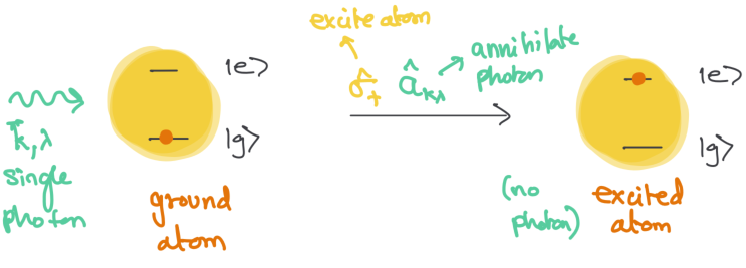
\includegraphics[width=\columnwidth]{PartOne/ChapterFour/figures/quantizedenergylevelatom_firstterm.png}
        \caption{First term}
    \end{subfigure}
    \hfill
    \begin{subfigure}{.45\columnwidth}
        \centering
        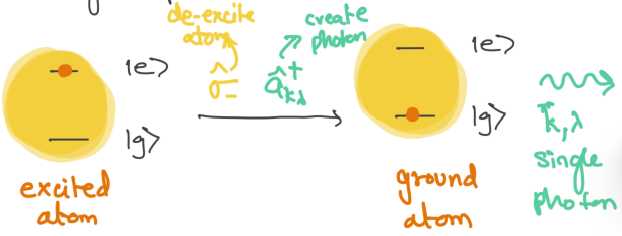
\includegraphics[width=\columnwidth]{PartOne/ChapterFour/figures/quantizedenergylevelatom_secondterm.png}
        \caption{Second term}
    \end{subfigure}
    \caption{Process of interaction light-matter.}
\end{figure}